\chapter{Evaluation}

\section{Purpose of Evaluation}


\section{Internal Test}

\subsection{Evaluation Plan}

\subsection{Results}


\section{User Test}

\subsection{Evaluation Plan}

When conducting this user test, it is the intention to get some data from the users about the different effects and gestures. 
Initially, the users are asked to sign a consent form, see Appendix \ref{Consent} and \ref{Script} for script and consent form. They are then told to put on the glove and try to apply the effects. Afterwards, they are then asked to answer a questionnaire, see Appendix \ref{Questionnaire}. 

\subsection{Apparatus and Setup}



\begin{minipage}{\linewidth}% to keep image and caption on one page
\makebox[\linewidth]{%        to center the image
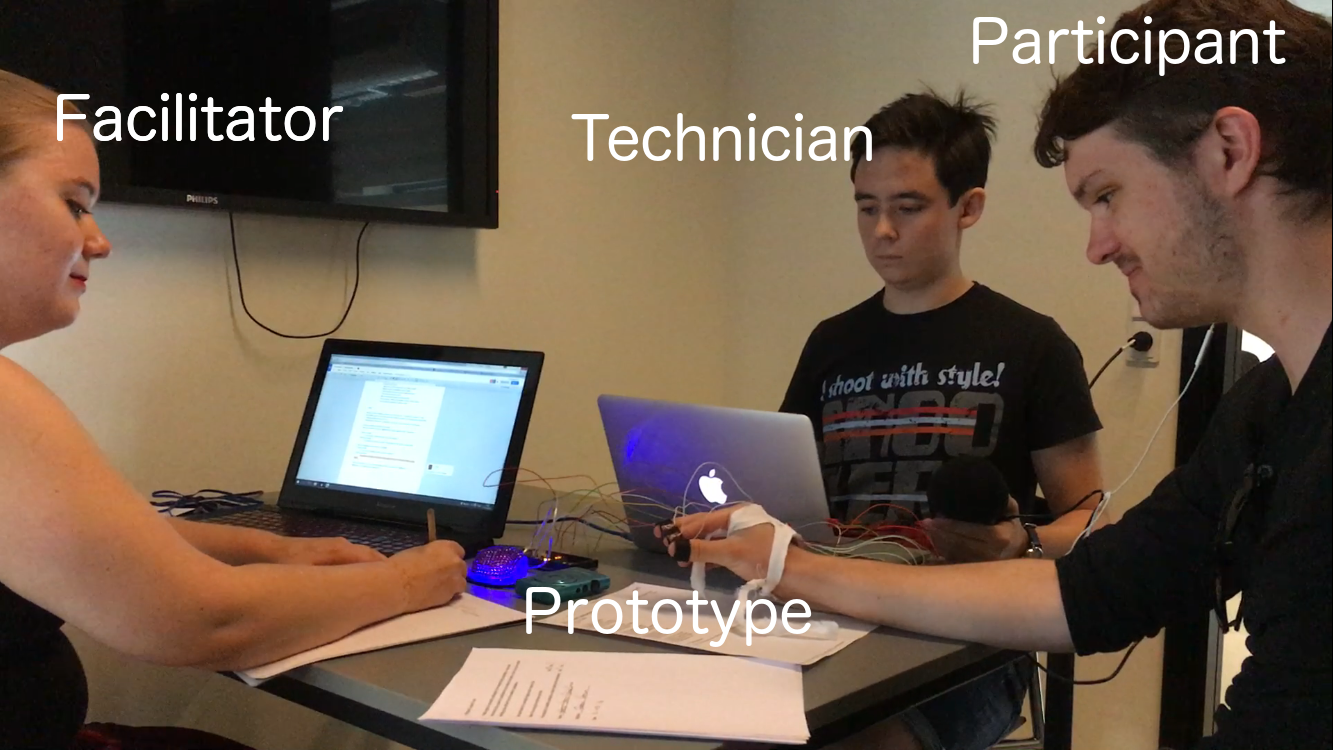
\includegraphics[keepaspectratio=true,scale=0.8]{Setup}}
\captionof{figure}{The Test Setup}\label{Setup}
\end{minipage}\\

\subsection{Results}


\section{Analysis}

\subsection{Theory}

\subsection{Results}


\section{Conclusion}